\documentclass{article}
\usepackage[letterpaper,margin=1in]{geometry}
\usepackage{xcolor}
\usepackage{fancyhdr}
\usepackage{tgschola} % or any other font package you like
\usepackage{graphicx,subfigure, subcaption}
\usepackage[sorting=none]{biblatex} %Imports biblatex package

\addbibresource{reference.bib}

\def\system{RealityCanvas}
\pagestyle{fancy}
\fancyhf{}
\fancyhead[C]{%
  \footnotesize\sffamily
  \yourname\quad
  web: \textcolor{blue}{\itshape\yourweb}\quad
  \textcolor{blue}{\youremail}}

\newcommand{\soptitle}{Statement of Purpose}
\newcommand{\yourname}{Zhijie Xia}
\newcommand{\youremail}{zhijie.xia@ucalgary.ca}
\newcommand{\yourweb}{https://www.zhijiexia.org/}

\newcommand{\statement}[1]{\par\medskip
  \underline{\textcolor{blue}{\textbf{#1:}}}\space
}

\usepackage[
  colorlinks=false,
  breaklinks,
  pdftitle={\yourname - \soptitle},
  pdfauthor={\yourname},
  unicode
]{hyperref}


\begin{document}

\begin{center}\LARGE\soptitle\\
\large \yourname\ , M.Sc Computer Science (Thesis), Robotics - Fall 2024
\end{center}

\hrule
\vspace{1pt}
\hrule height 1pt

\bigskip

I am writing to express my interest in pursuing a Master of Science in Computer Science (Thesis) at McGill University, 
focusing on Robotics. My primary research interests include Deep Reinforcement 
Learning and Robot Control for real-world applications, with the goal of leading a team to create fully autonomous robots.


My first experience with research occurred during an internship at the Programmable Reality Lab at University of Calgary 
after my third year of undergraduate studies. I was fascinated by sketching in AR as it is
a very intuitive way of creating virtual objects and wanted 
to make it more expressive and dynamic. 
My research interests were further developed when I worked on a research project with Dr. Ryo Suzuki. 
This was the "RealityCanvas" project, an authoring tool designed to facilitate the creation
of improvised scribble animation in an augmented environment~\cite{xia2023realitycanvas}.
I curated a dataset comprised of videos and images sourced from different social media platforms.
These contained scribble animations edited using context creation software like Adobe After Effects and Adobe Premiere Pro. 
This dataset served as the foundation for taxonomy analysis, in which I systematically catergorized
six animation techniques. Motivated by the taxonomy analysis,
I developed a web application that allows users to generate scribble animation using the six common techniques. 
Users can draw these animations directly onto the screen and apply them to the video stream. The workflow 
is shown shown in Figure \ref{fig:teaser}. In addition to designing and implementing the system, I conducted a user study to access its usability and expert
interviews to evaluate its effectiveness. The results of the user study demonstrated that the system facilitates
easy and spontaneous animation creation. Expert interviews further affirmed the system's effectiveness in generating 
scribble animations.


\begin{figure}[h!]
  \centering
  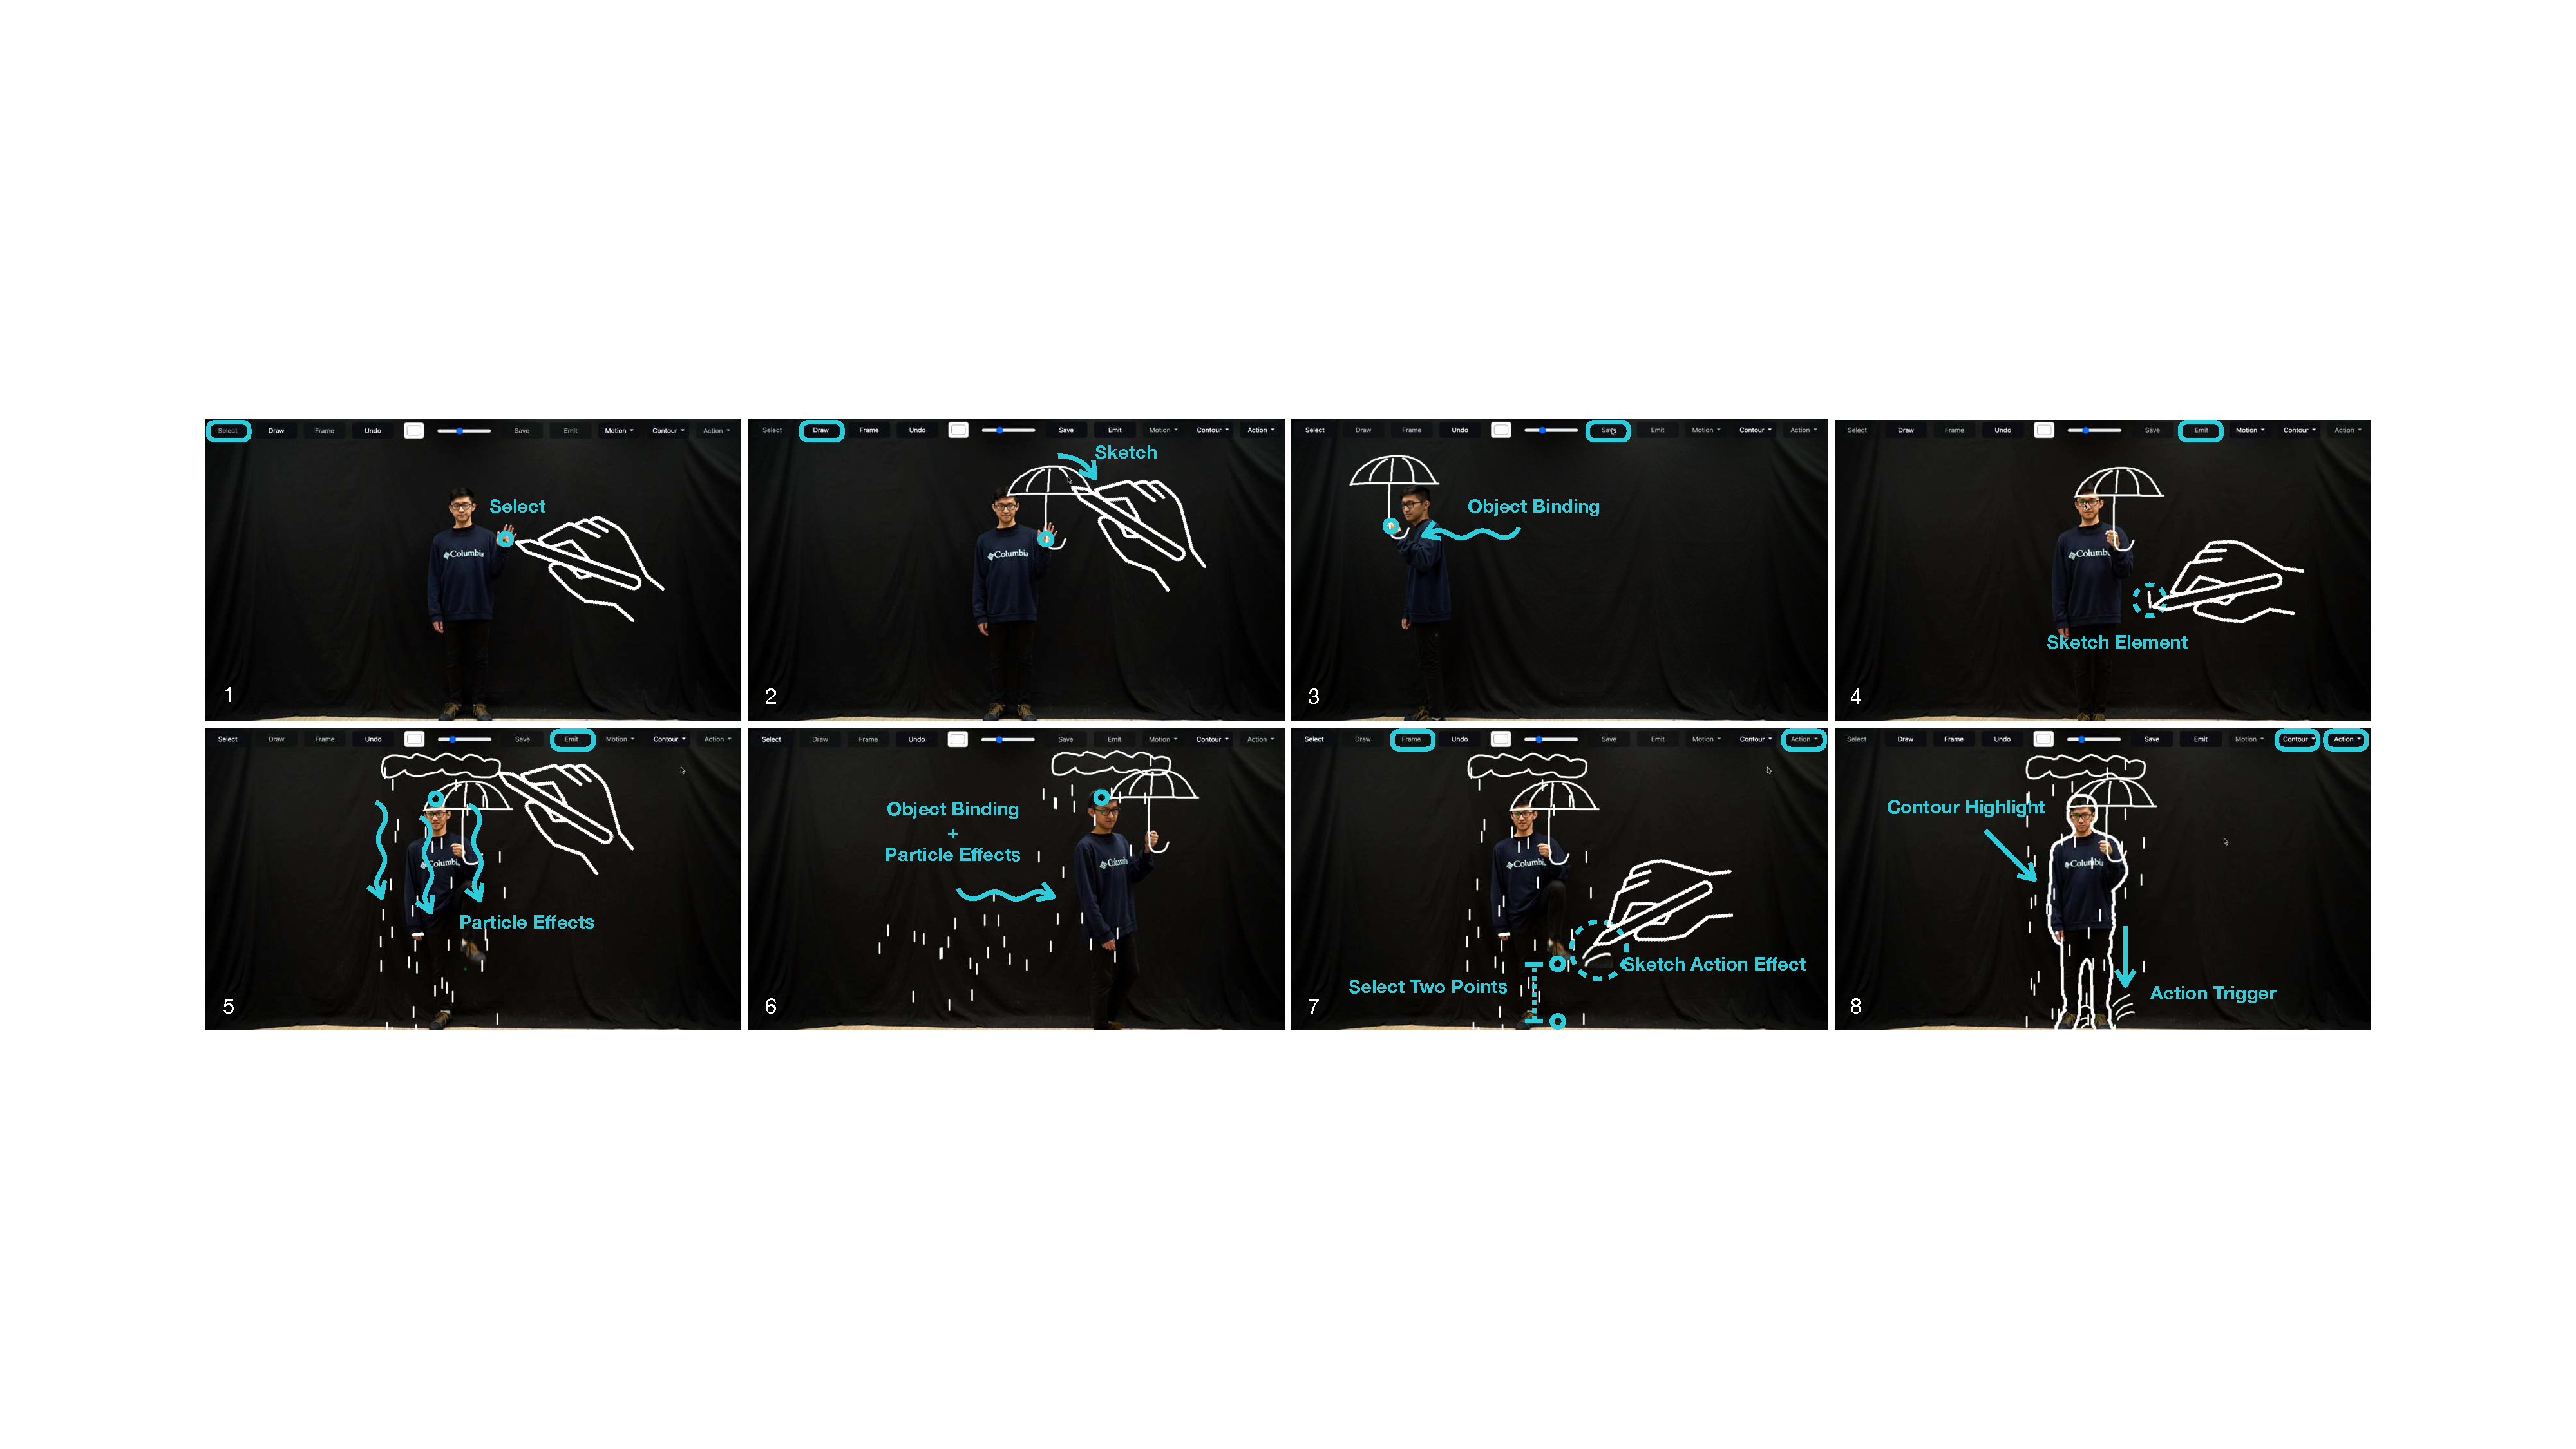
\includegraphics[width=\textwidth]{figures/teaser-num.pdf}
  \caption{\system{} workflow (from top left to bottom right): 1) select a hand as a tracking point, 2) sketch an umbrella bound to the hand, 3) the umbrella moves when the hand moves, 4) sketch a raindrop, 5) draw a cloud as an emitter line to show particle effects, 6) the cloud also moves with object binding, 7) select the ground and right foot then sketch a water splash, 8) show the water splash and contour highlight based on the stomp action.}
  \label{fig:teaser}
\end{figure}


During this internship, I have had the valuable opportunity to immerse myself in academic research, igniting my passion for 
applied research and computer science. I am deeply intrigued by the process of transforming ideas into real-world applications.
Working alongside Dr. Suzuki and his team, I came to realize that the world is constant state of flux, with perpetual challenges 
and uncharted ideas awaiting exploration. Even when addressing the same problem, there exist innovative approaches to tackle it, 
challenging established conventional solutions. During this internship, I navigated the entire academic research publication process, 
from conducting literature reviews and implementing the system to submitting the paper, 
addressing peer-review feedback, and achieving publication. 
The paper titled "RealityCanvas: Augmented Reality Sketching for Embedded and Responsive Scribble Animation Effects" [1], 
with me as the first author, was published at UIST 2023. This experience introduced me to academic research and fueled my enthusiasm 
for developing my research skills.


After my internship at Programmable Reality Lab, I initiated an independent research project with Dr. Joel Reardon for my undergraduate thesis,  
aimed at investigating the Android permission system's design and its role in the 
prevalence of overpriviledged apps. The transition from HCI to security research is both 
challenging and fulfilling. I conducted literature reviews and 
made significant refinements to the 
state-of-the-art API permission mappings, as discussed in prior research~\cite{felt2011android,au2012pscout}. 
Furthermore, I developed pipeling to build APK and API permission usages corpus by downloding apks from Google Play and 
reverse engineering them into smali package. I explored several frequent itemset mining algorithm 
and applied FP-growth~\cite{borgelt2005implementation} mapping to uncovered the permission usage patterns. 
35,117 Android applications sourced from the Google Play Store and an API-permission mapping, 
comprising 1,976 API calls and 323 permissions. We suspected potential maliciousness of certain 
patterns. Notably, we uncovered instances where applications exploited the 
combination of \textit{SET\_EXACT\_ALARM} and \textit{ACCESS\_FINE\_LOCATION} to periodically transmit device location 
data to external servers. Due to time constraints and personal challenges, we couldn't conduct a more thorough 
investigation of these potentially malicious apps or prepare them for peer review. 
This experience marked my entry into security research, 
enhancing my skills and fueling my determination to address existing vulnerabilities in the field.

After joining Knowd AI, a venture-capital funded startup in Toronto, 
I focused on research and development for Knowd board, the company's flagship product.
Leveraging my previous work on "RealityCanvas," I designed an intuitive workflow for non-technical users, 
including drag-and-drop functionality, automatic clustering, and summarization features. 
I also improved the user interface for a more modern and user-friendly experience, 
informed by my research and user studies.
Furthermore, I conducted extensive research and integrated 
BERTopic~\cite{BERT} to support Knowd board's development, aligning 
with our MVP's requirements and contributing to its success. 
Currently, I'm a firmware developer at Lucid Vision Labs, Inc in Vancouver, 
where I transitioned from software to firmware development. This move reflects 
my desire for new challenges and expertise in camera systems and computer vision. 
My responsibilities include designing firmware for next-generation GigE cameras and 
developing a reporting suite for the manufacturing and testing team, expanding my industry expertise.

Throughout my journey, which spans from my undergraduate studies and research to my current 
industrial co-op experience, my determination and passion for pursuing academic research in graduate school 
have significantly intensified. I am drawn to the field of robotics for a profound reason: I envision a future 
where robots are not only ubiquitous but also indispensable in our daily lives. This vision has been a 
driving force since my early interest in robotics and my self study on the literature of deep reinforcement 
learning. I am motivated by the desire to create tangible 
solutions that can interact physically with the real world, rather than 
limiting my impact to SaaS products or mobile applications where only reside in virtual space.
I find various aspects of computer science fascinating, such as human-computer interaction, security, 
computer vision, and machine learning. The field of robotics stands out as particularly promising to me 
because it combines these interests and has the potential to make a significant real-world impact due to 
its multi-disciplinary nature.


With the respect to my thesis, I am eager to partner with and benefit from the expertise of 
Dr. Gregory Dudek, Dr. David Meger and/or Dr. Doina Precup's due to my deep interest in the projects undertaken by 
the Mobile Robotics Lab. Along with this, I find Dr. Gregory Dudek
and Dr. David Meger's work "Towards Autonomous Robotic Coral Reef Health Assessment"~\cite{manderson2016towards}
and "Learning to Drive Off Road on Smooth Terrain in Unstructured Environments Using an On-Board Camera and Sparse Aerial Images"~\cite{manderson2020learning}
particularly captivating that are examples of how robots can be used to solve real world problems in cross-disciplinary domains.
Dr. Doina Precup's research, as demonstrated in 'Deep Reinforcement Learning That Matters'~\cite{henderson2018deep}, greatly interests me 
because it addresses the crucial aspects of reproducibility and the advancement of deep reinforcement learning research, 
which aligns with my own values.

% I would like to conclude with a quote from Dr. Ryo Suzuki's enlightening public talk at the Calgary Public Library:

% "When the first messaging machine was invented in the latter part of the last century, people were astonished 
% by a machine that could send messages. Then came the invention of the first mobile phone, 
% and people marveled at a device that could transmit voice on a handheld gadget. Subsequently, 
% the iPhone and the advent of so-called smartphones captivated us with machines we could touch. 
% We have witnessed these profound changes. Nowadays, even six-year-olds instinctively touch every screen they encounter, 
% assuming it to be touch-sensitive. In essence, we are all digital immigrants in a rapidly evolving world. We have a choice: 
% embrace this change and contribute to making the world a better place, or ignore it and risk being left behind."

% For me, the choice is clear—I choose to wholeheartedly embrace this change.
% Beyond mere acceptance, my unwavering commitment lies in addressing the flaws within our world 
% and tirelessly working towards crafting tangible solutions.
% My focus centers on the development of autonomous robotics systems with the capacity to 
% drive substantial impact. Simultaneously, I am determined in pushing the boundaries of what is 
% achievable in our physical reality. Through these efforts, I aspire to make a meaningful contribution 
% to the progress of our global community as a dedicated graduate researcher in the field of robotics.

Accepting my admission would welcome a passionate and dedicated researcher with a strong background 
and a history of achievements into your program. 
I am confident in my ability to contribute significantly to the Mobile Robotics Lab 
and am eager to engage actively in its research initiatives. 
Furthermore, I look forward to collaborating with the esteemed 
faculty and fellow students to advance robotics and make a meaningful global impact.

\printbibliography
\end{document}
